\section{Introduction}
The register-transfer level (RTL) programming model paved the road for Verilog and VHDL to flourish as the leading hardware description languages (HDLs). That road, however, is steadily nearing its end as both hardware designs and devices become increasingly more complex. While the software world is striving for a "write once, run anywhere" programmability, the complexity of an RTL design implementing a given functionality may vary greatly across different FPGA and ASIC devices that incorporate various technologies and core components. Moreover, minor requirement changes may lead to significant redesigns, since RTL abstraction tightly couples functionality with timing constraints. For example, registers serve various roles such as preserving a state, pipelining and balancing a data path, deriving timed signals from an input clock, and synchronizing an input signal. This coupling between functionality, timing constraints, and device constraints leads to verbose and unportable RTL designs. 

Ongoing efforts to bridge this hardware programmability gap~\cite{Kapre2016, Nane2016, Windh2015} can be largely split into two classes: high-level synthesis (HLS) tools and high-level RTL (HL-RTL) languages.
On the one hand, HLS tools (such as Vivado~\cite{Vivado2012}, Catapult~\cite{graphics2008catapult}, and others~\cite{Kavvadias2013, synphony2015}) rely on programming languages like C and incorporate auto-pipelining and optimization mechanisms to make hardware accelerators accessible for non-hardware engineers. While this approach is successful in algorithmic acceleration domains, such languages carry von Neumann sequential semantics and thus hinder construction of parallel hardware, which is crucial for hardware design~\cite{Zhao2017}. Moreover, some trivial periodic hardware operations (like toggling a LED) are unbearably difficult to implement in HLS languages.
On the other hand, HL-RTL languages (such as Chisel~\cite{Bachrach2012}, Bluespec~\cite{nikhil2004bluespec}, PyRTL~\cite{Clow2017}, and others~\cite{Charles2016, Liu2017, jiang2018mamba, decaluwe2004myhdl, CxLang2014, Lockhart2014}) aim to enhance productivity by introducing new hardware generation constructs and semantics but do not abstract away register-level description (even Bluespec, which uses concurrent guarded atomic actions, assumes rules complete within a single clock cycle). Therefore, HL-RTL designs are still subjected to the \emph{"tyranny of the clock"}~\cite{Sutherland2012} and are bound to specific timing and target constraints.

In this paper we propose dataflow-based HDL constructs that abstract away registers and clocks. We further introduce DFiant\footnote{A preliminary version of DFiant was first introduced as a poster. The reference was removed for blind review.}, a Scala-embedded HDL that utilizes these dataflow constructs to decouple functionality from implementation constraints. DFiant brings together constructs and semantics from dataflow\cite{le1986signal, Thuau1991, gurd1985manchester, arvind1992id}, hardware, and software programming languages to enable truly portable and composable hardware designs. The dataflow model offers implicit concurrency between independent paths while freeing the designer from explicit register placement that binds the design to fixed pipelined paths and timing constraints.  

\begin{figure*}[t]
	\centering
	\captionsetup{justification=centering}
	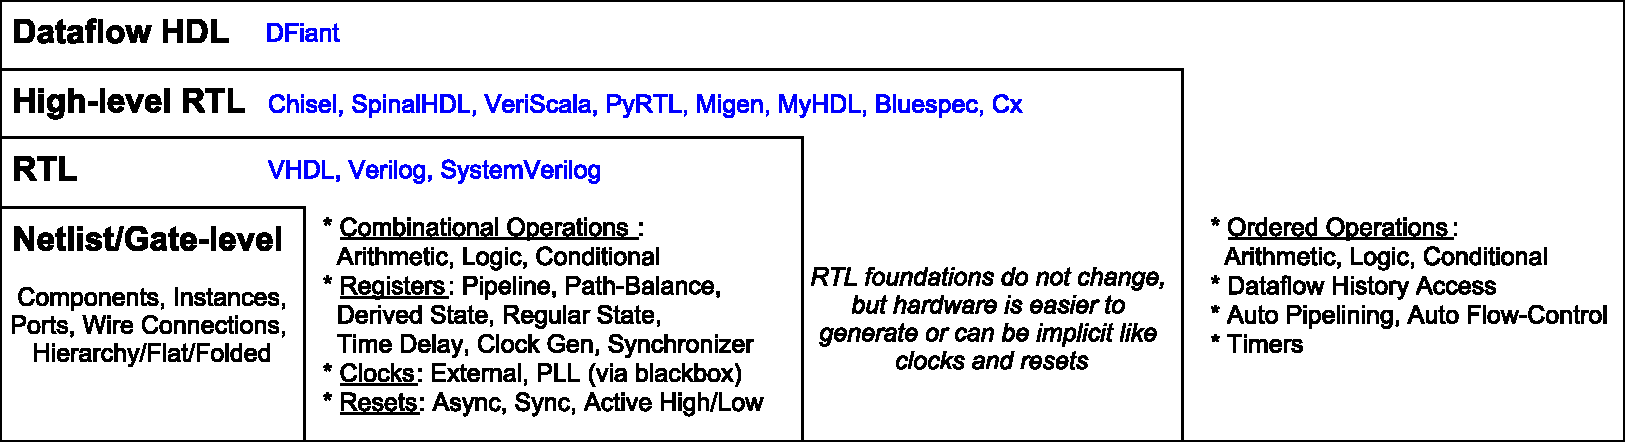
\includegraphics[width=\linewidth]{graphics/motivation.pdf} 
	\captionof{figure}{HDL abstraction layer summary (lowest=netlist, highest=dataflow)\\ Each layer subsumes the capabilities of the layer below it. Dataflow constructs replace RTL registers with their true functionality (e.g., state) or inserts them implicitly (e.g., pipelining) }
	\label{fig:motivation}
\end{figure*}

Recent related dataflow-for-hardware efforts are the Maxeler framework~\cite{Pell2011} and its MaxJ Java-based programming language, the OpenDF framework~\cite{bhattacharyya2008opendf} which is based on the CAL actor language~\cite{eker2003cal}, and CAPH~\cite{serot2011implementing}. MaxJ indeed shares common traits with DFiant, but it is tailored for its target hardware framework and is not designed to be a general purpose HDL. Both OpenDF and CAPH share similar goals with our work, but they use actors and networks to describe hardware, which is completely different than a conventional HDL composition based on component instances and port connections.

This work focuses on applying dataflow principles through the DFiant language and compiler. DFiant is \emph{not} an HLS language, nor is it an RTL language. Instead, DFiant is an HDL that provides abstractions beyond the RTL behavioral model, which reduce verbosity and maintain portable code. Since DFiant is implemented as a Scala library, it offers a rich type safe ecosystem alongside its own hardware-focused type system (e.g., bit-accurate dataflow types, input/output port types). The library performs two main tasks: first, the frontend compilation, which enforces the type-safe rule-system and constructs a dataflow dependency graph; and second, the backend compilation, which translates the graph into a pipelined RTL code and a TCL constraints file. The resulting code can be synthesized using commercial tools. 

The remainder of this paper is organized as follows. The next section details the motivation behind the dataflow HDL abstractions, and Section~\ref{sec:dfiant} which provides a general overview of the DFiant HDL language. 
Section~\ref{sec:evaluation} describes our evaluation of the DFiant language and compiler, and, finally, Section~\ref{sec:conclusion} concludes the paper.


%Interactions between DFiant types lead to hardware construction, while non-DFiant types (e.g. Integer) are considered as constants. 
 